\section{Auftrag}
\label{sec:generalProvision}


Im Rahmen dieser Semesterarbeit soll eine Lösung zur oben beschriebenen Problematik ausgearbeitet werden. Der Fokus liegt auf der Erstellung eines autarken Anzeigesystems welches über eine drahtlose Schnittstelle bedient werden kann. Die folgende Punkte sollen dabei abgearbeitet werden:
\begin{itemize}
	\item Recherche bezüglich Schnittstelle und Energy Harvesting.	
	\item Vor- und Nachteile bestehender Technologien abwägen und geeignete Hardware wählen.	
	\item Erstellen eines lauffähigen Prototypen.
\end{itemize}

\begin{figure}[h]
	\centering
	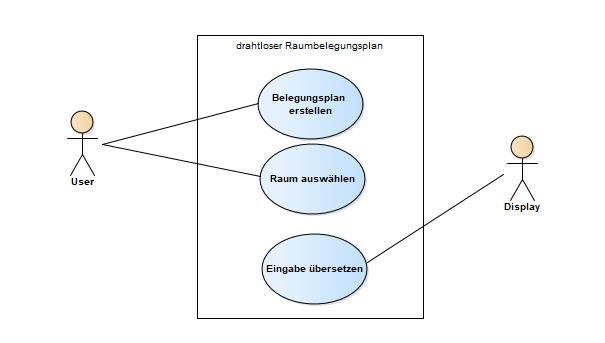
\includegraphics[width=0.8\textwidth]{./Use-Case-Model.png}
	\caption{Use-Case Diagramm\label{use-case}}
\end{figure}

Der Prototyp richtet sich nach dem Use-Case Diagramm in Abbildung \ref{use-case}.